\documentclass[a4paper, 11pt]{article}
\usepackage{comment} 
\usepackage{fullpage}
\usepackage{hyperref}
\usepackage{amsmath}
\usepackage{environ}
\usepackage{tabto,enumitem}
\usepackage{lipsum}
\usepackage{float}
\usepackage{tabto}
\usepackage{booktabs} 
\usepackage{graphicx}
\usepackage{graphics}

\usepackage[ruled]{algorithm2e}
\renewcommand{\algorithmcfname}{ALGORITHM}

\begin{document}
\noindent
\large\textbf{Deliverable 1} \hfill \textbf{Rahul Sharma} \\
\normalsize SOEN 6011 \hfill \textbf{40020034} \\
Function 6 :  $f(x)= ab^x$  \hfill Date: 18/07/2019 \\

\section*{Problem 1}
\section{Introduction}

F6:  $f(x)= ab^x$ is a exponential function where a is a constant, b is a base and x is a exponent or power. Here, x is a  real variable. This function is one of the most commonly used function in mathematics.

\section{Domain \& Co-Domain}

\subsection{Domain}
\begin{itemize}
  \item it includes all the real numbers. \\
   To be specific,  For  $ b > 0$ ,  $x \in R$	
 \end{itemize}
  
 \subsection{Co-Domain}
 \begin{itemize}
  \item  $For$ $ b > 0$ , range is $[0,\infty)$  where $ b \in R$  and  $x \in R$. 
  \item  $For$ $ b = 0$ and $y =0$, range is 1 and  $For$ $ b = 0$ and $x>0$, range is 0.
 \item  $For$ $ b < 0$ , range is $(-\infty,\infty)$  where $ b \in R$  and  $x \in Z$ $^{[1]}$.
\end{itemize}
 \subsection{Restrictions}
 \begin{itemize}
  \item  a cannot be zero
\end{itemize}

\section{Characteristics}

\begin{itemize}
  \item $\boldsymbol{Growth}$ : When $b > 0$, the function is called an exponential growth function. It can be seen on the left side of figure 1$^{[2]}$.

  \item $\boldsymbol{Decay}$ : When $b < 0$, the function is called an exponential decay function. It is shown on the right hand side of the graph.
  
  \item $ \textbf{Injectivity \& Surjectivity}$ : This function is not injective which means it is not one-to-one function but it is surjective which means it is onto function.
  
   \item $\boldsymbol{Commutativity}$:  This function is not commutative which means $x^y \ne y^x $ for $x\ne y$.
  \begin{figure}[H]
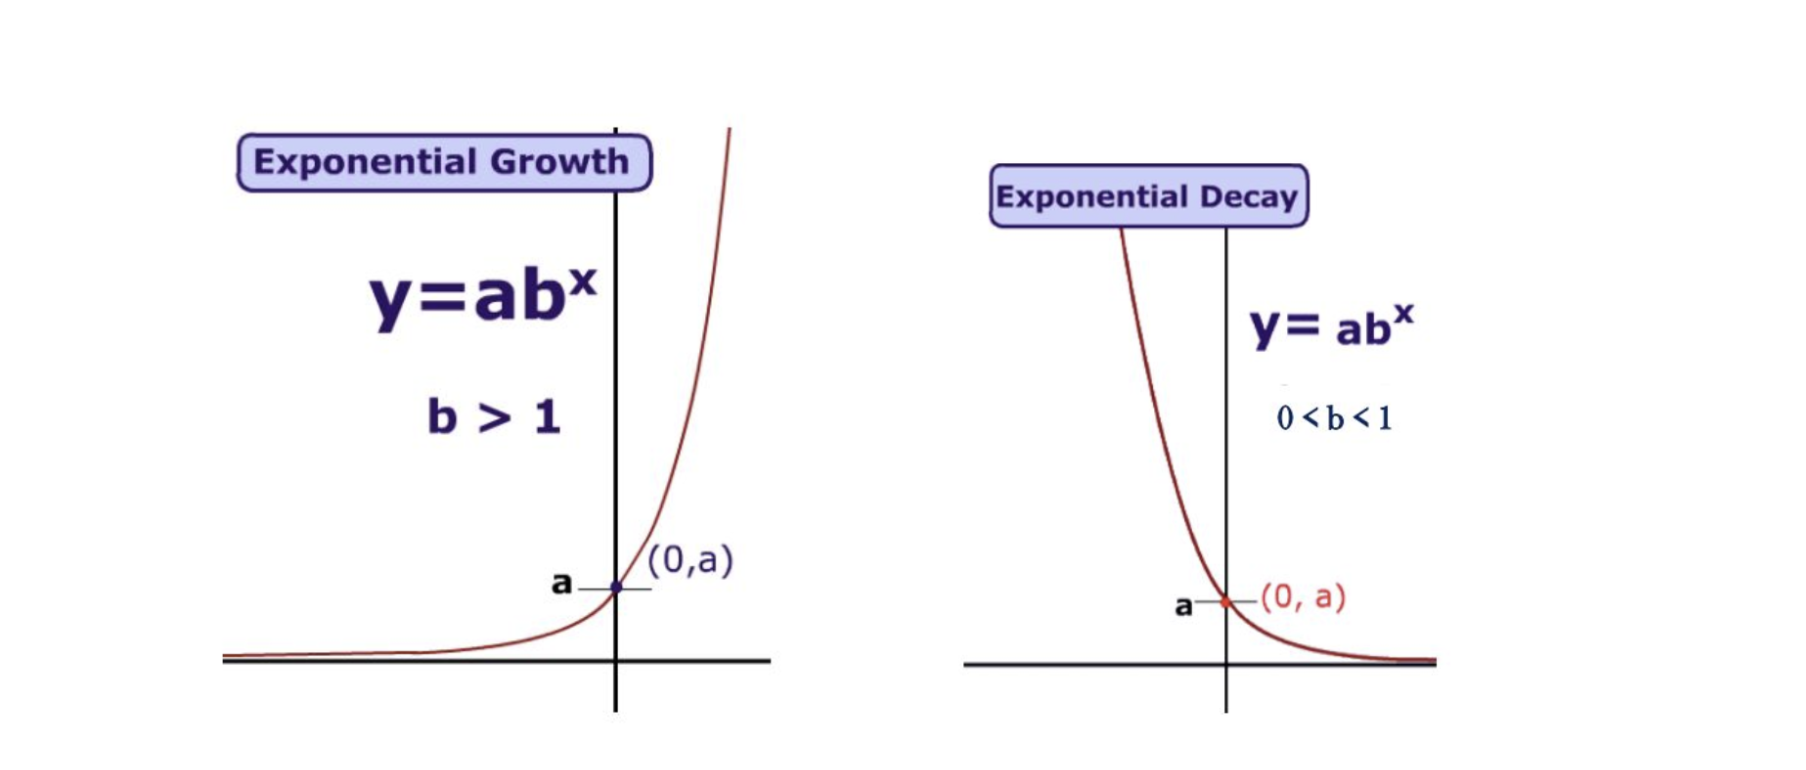
\includegraphics[width=18cm]{exp.png}
\caption{Exponential growth and Exponential Decay graph}
\label{exp}
\end{figure}
\end{itemize}

\newpage
\section*{Problem 2}
\section*{Requirements}
    \subsection*{First Requirement}
    \begin{itemize}
        \item \textbf{ID = } FR1
        \item \textbf{Type = } Functional Requirements
        \item \textbf{Version = } 1.0
        \item \textbf{Difficulty = } Easy
        \item \textbf{Description = }System shall take an input x, b and a  to give an output of $ab^x$ function.\\
        Example :for  $x = 2, b = 1, a = 1 $ , $ ab^x = 1$
    \end{itemize}
    \subsection*{Second Requirement}
    \begin{itemize}
        \item \textbf{ID = } FR2
        \item \textbf{Type = } Functional Requirements
        \item \textbf{Version = } 1.0
        \item \textbf{Difficulty = } Easy
        \item \textbf{Description = } $ab^x$ function does not depend on any other function.\\
    \end{itemize}
    \subsection*{Third Requirement}
    \begin{itemize}
        \item \textbf{ID = } FR3
        \item \textbf{Type = } Functional Requirements
        \item \textbf{Version = } 1.0
        \item \textbf{Difficulty = } Easy
        \item \textbf{Description = }  User shall give an input from all real numbers for x.  
    \end{itemize}
    \subsection*{Fourth  Requirement}
    \begin{itemize}
        \item \textbf{ID = } FR4
        \item \textbf{Type = } Functional Requirements
        \item \textbf{Version = } 1.0
        \item \textbf{Difficulty = } Easy
        \item \textbf{Description = }when user gives other input then integer that is string then system shall not accept and should show input not properly defined.  
    \end{itemize}
        \subsection*{Fifth  Requirement}
    \begin{itemize}
        \item \textbf{ID = } FR5
        \item \textbf{Type = } Functional Requirements
        \item \textbf{Version = } 1.0
        \item \textbf{Difficulty = } Easy
        \item \textbf{Description = }when user gives doesn't specify all three inputs a, b and x, the system should not accept and should throw an error.
    \end{itemize}

\newpage
\section*{Problem 3}
\section*{Pseudocode and Algorithm}
Calculate: $y = ab^x$

\begin{algorithm}
\caption{Iterative algorithm to calculate $ab^x$}
\begin{algorithmic} 
1. function \textbf{exponent\_iterative(a,b,x)}\\
\textbf{in: } double number x, a, b\\
\textbf{out: } double number sum\\
2. \STATE $sum \leftarrow 1$\\
3. \STATE $temp \leftarrow 1$\\
4. for {$temp \leq x$} do\\
5.\qquad \STATE $sum \leftarrow sum*b$\\
6.\qquad\STATE $temp \leftarrow temp+1$\\
7. end for \\
8. \STATE $sum \leftarrow sum*a$\\
9. \STATE return sum\\
\end{algorithmic}
\end{algorithm}
We keep track of our result in a variable called sum, which is initially equal to 1. Then we loop from 1 to x number of times, incremented by one on each iteration and on each iteration we multiply sum by b. At the end of the loop value of sum is equal to $b^x$. At the last step we return our desired result of $a * sum$.
\newpage
\begin{algorithm}
\caption{Recursive algorithm to calculate $ab^x$}
\begin{algorithmic} 
1. function \textbf{exponent\_recursive(a,b,x)}\\
\textbf{in: } double number x, a, b\\
\textbf{out: } double number result\\
3. \STATE $power \leftarrow exponent\_helper(b,x)$\\
4. \STATE $result = power * a$\\
5. return result
\end{algorithmic}
\end{algorithm}
\begin{algorithm}

\begin{algorithmic} 
1. function \textbf{exponent\_helper(b,x)}\\
\textbf{in: } double number x, b\\
\textbf{out: } double number sum\\
2. if  \STATE $x < 0$  then\\
3. \qquad $b \leftarrow 1.0 / b$ \\
4. \qquad $x \leftarrow -x$ \\
5. \qquad return $exponent\_helper(b, x)$ \\
6. else if \STATE $x = 0$ then \\
7.    \qquad return $1.0$ \\
8. else if \STATE $x = 1$ then \\
9.    \qquad return b \\
10. else if \STATE $x \mod  2 = 0$ then \\
11.    \qquad $b \leftarrow b * b$ \\
12.    \qquad $x \leftarrow x / 2$ \\
13.    \qquad return $exponent\_helper(b, x)$\\
14. else \\
15.    \qquad $b \leftarrow b * b$ \\
16.    \qquad $x \leftarrow x - 1$ \\
17.    \qquad $x \leftarrow x / 2$ \\
18.    \qquad return $exponent\_helper(b, x)$\\
19. end if \\
\end{algorithmic}

\end{algorithm}
We define a helper function called exponent\_helper which calculates $b^x$. In the base case when $x = 0$, we return 1, otherwise when $x = 1$ we return b. When x is even we recurse on $b = b* b$ and $x = x /2$. In case when x is odd we recurse on $ b = b* b$ and $x = (x-1)/ 2$. In the end, in our main function exponenet\_recursive we multiply the result of exponent\_helper to the value of a and return our result.

\newpage

\subsection*{Advantages and Disadvantages}
\subsubsection*{Algorithm 1:}
Advantages:\\
1. In terms of space complexity, iterative algorithms don't suffer from stack overflow because all operations are done on the heap. \\
2. They are fairly intuitive to read and follow for human beings.\\
Disadvantages:\\
1. The time complexity of the iterative algorithm is $O (n)$, hence it is not very efficient for larger inputs in terms of time.  \\
2. Proper terminating condition for loop is needed or else we might get stuck in infinite loop.
\subsubsection*{Algorithm 2:}
Advantages: \\
1. The time complexity of our recursive algorithm is $O (log n)$. Our version of recursive algorithm is optimized and tail recursive so that we don't get stack overflow error. So even for large inputs, it handles it very well. \\
2. Recursion has higher maintainability than loop. There's little to no modification needed if we handle base case correctly\\
Disadvantages:\\
1. When using recursion, it needs system continuously allocates memory space, thus it has a bad effect on efficiency leading to stack overflow. \\
2. The algorithm is difficult to understand, especially for edge cases and it is very easy to make mistakes in handling base case. 
3. It is not really very readable.
\subsubsection*{Conclusion}
My decision is to go with the recursive algorithm mostly because of the time complexity of the algorithm. The calculator should give result to the user in fairly less time and given the option between iterative and recursive solution, recursive would definitely perform well. 

\begin{thebibliography}{9}
\bibitem{MathBitsNotebook}
MathBitsNotebook,\\
\url{https://mathbitsnotebook.com/Algebra1/FunctionGraphs/FNGTypeExponential.html}
\bibitem{TutorialsPoint}
TutorialsPoint,\\
\url{https://www.tutorialspoint.com/java/lang/math_pow.htm}
\bibitem{R. T. Barker and D. W. Biers} R. T. Barker and D. W. Biers,   "Software usability testing: Do user self-consciousness and the laboratory environment make any difference?" in Part 2 (of 2), October 24, 1994 - October 28, 1994, .
\bibitem{S. L. Sparagen and A. Riback}  S. L. Sparagen and A. Riback, "Flexible software interface design," Ergonomics Des., vol. 7, (4), pp. 4-8, 1999.
\bibitem{M. Hon, G. Russell and M. Welch} M. Hon, G. Russell and M. Welch, "Open source software considerations for law enforcement," IT Professional, vol. 12, (6), pp. 18-23, 2010. Available: http://dx.doi.org/10.1109/MITP.2010.121. DOI: 10.1109/MITP.2010.121.
\bibitem{J. Ragot, D. Maquin and A. Kondo} J. Ragot, D. Maquin and A. Kondo, "Control design for loop transfer recovery," in Part 1 (of 3), October 2, 1994 - October 5, 1994, .
\bibitem{B. Haberman and H. Averbuch} B. Haberman and H. Averbuch, "The case of base cases: Why are they so difficult to recognize? student difficulties with recursion," in ITiCSE 2002 - Proceedings of the 7th Annual SIGCSE Conference on Innovation and Technology in Computer Science Education, June 24, 2002 - June 28, 2002, Available: http://dx.doi.org/10.1145/544414.544441. DOI: 10.1145/544414.544441.
\end{thebibliography}

\end{document}
 
